\documentclass[../main]{subfiles}
\usepackage{lastpage,xr,refcount,etoolbox}
%\externaldocument{../Appendices/Appendix1-CodigosBase}
\begin{document}


\chapter{Testing and Extras}

{
\hypersetup{linkcolor=black}
\minitoc
\vspace{5mm}
}

We have already explored the process of defining a neural network and how it uses calculus to learn classification tasks from data. With this knowledge, we were able to implement our own neural network in raw Python. An important next step is to test how well our neural network performs on a given task.

\section{Handwritten digits classification}
Once you have a trained neural network, you can use it for a multitude of tasks. One very popular and historically significant application is the recognition and classification of handwritten digits. To achieve this, we need to train our neural network using thousands of correctly labeled examples, and then evaluate its performance on a separate set of test data.

\subsection{The python script}
For this purpose, the MNIST dataset provides a comprehensive collection of 60,000 labeled training images of handwritten digits and 10,000 test images. We will create a short Python script to test our neural network and explain how we can adjust different hyperparameters to improve the model’s accuracy:

\begin{lstlisting}
import numpy as np
import tensorflow as tf
import network1 as nt
import os

def load_data_wrapper(num_samples=60000):
    # Download the MNIST dataset
    (x_train, y_train), (x_test, y_test) = tf.keras.datasets.mnist.load_data()


    indices = np.random.choice(x_train.shape[0], num_samples, replace=False)
    x_train_sample = x_train[indices]
    y_train_sample = y_train[indices]

    training_inputs = [np.reshape(x, (784, 1)) for x in x_train_sample]
    training_results = [vectorized_result(y) for y in y_train_sample]
    training_data = list(zip(training_inputs, training_results))

    test_inputs = [np.reshape(x, (784, 1)) for x in x_test]
    test_data = list(zip(test_inputs, y_test))

    return (training_data, test_data)

def vectorized_result(j):
    """Return a 10-dimensional unit vector with a 1.0 in the jth
    position and zeroes elsewhere.  This is used to convert a digit
    (0...9) into a corresponding desired output from the neural
    network."""
    
    e = np.zeros((10, 1))
    e[j] = 1.0
    return e

def main():
    os.environ['TF_ENABLE_ONEDNN_OPTS'] = '0'

    network = nt.Network([784, 30, 10])
    (training_data, test_data) = load_data_wrapper()
    
    network.SGD(training_data, 40, 5, 0.1, test_data=test_data)
    
if __name__ == "__main__":
    main()
\end{lstlisting}

Once we have the script, there are two important considerations. First, backpropagation is a computationally expensive and slow algorithm due to the NP-completeness of the problem. Training the network on all 60,000 training inputs for multiple epochs involves millions of operations and multiplications, which can take several minutes to compute. To speed up the process, you can reduce the number of training inputs or epochs, but be aware that this may also decrease the accuracy of the model.

Second, there are several hyperparameters of the network that we can adjust to improve its accuracy. These include the mini-batch size, the number of epochs, the learning rate, and the architecture of the network. For example, let’s try training the network with a learning rate of 0.01 (instead of 3, which is typically too high) and keep the other parameters as shown in the code above:
\begin{lstlisting}
Epoch 0: 1754 / 10000
Epoch 1: 1285 / 10000
Epoch 2: 1341 / 10000
Epoch 3: 1275 / 10000
Epoch 4: 1669 / 10000
Epoch 5: 1589 / 10000
...
Epoch 33: 1605 / 10000
Epoch 34: 1598 / 10000
Epoch 35: 1603 / 10000
Epoch 36: 1711 / 10000
Epoch 37: 1679 / 10000
Epoch 38: 1727 / 10000
Epoch 39: 1711 / 10000
\end{lstlisting}
As you can see, the accuracy was very low compared to what we were hoping for. Let’s change the learning rate to 0.1 and see what happens:
\begin{lstlisting}
Epoch 0: 4306 / 10000
Epoch 1: 5477 / 10000
Epoch 2: 5029 / 10000
Epoch 3: 6322 / 10000
Epoch 4: 6606 / 10000
Epoch 5: 7229 / 10000
...
Epoch 33: 7791 / 10000
Epoch 34: 7587 / 10000
Epoch 35: 7616 / 10000
Epoch 36: 7478 / 10000
Epoch 37: 7553 / 10000
Epoch 38: 7482 / 10000
Epoch 39: 7494 / 10000
\end{lstlisting}
This time, the accuracy improved to nearly 80\%. Although there is still considerable room for improvement, the results are promising. I encourage anyone interested to experiment with other hyperparameters to achieve better performance. The key takeaway is that once you have the algorithm, it’s a matter of adjusting the parameters until it performs well for your specific use case.

\section{Extra considerations}
In the chapters where I explained the calculus behind neural networks, I consistently used the sigmoid function as the activation function and Mean Squared Error (MSE) as the loss function. However, nowadays, these are not the most commonly used choices for activation and loss functions due to the availability of more effective alternatives.

For loss functions, Cross-Entropy is often preferred over MSE, especially for classification tasks. Cross-Entropy is more suitable for classification because it directly measures the probability of class predictions and penalizes incorrect classifications more effectively. In contrast, MSE is more appropriate for regression tasks, as it does not handle probabilities and class boundaries well, which can lead to slower and less effective training for classification problems. The formula for Cross-Entropy is as follows:
\begin{equation*}
    C(a^l) = \frac{-1}{n} \cdot \sum_x [y^l\cdot ln(a^l)+(1-y^l)\cdot ln(1-a^l)]
\end{equation*}
If we differentiate this function, we can derive the formulas for the error, similar to how we did with the Mean Squared Error (MSE). This process will provide us with the formulas for the partial derivatives of the cost function with respect to the biases and weights. While I won’t go through the detailed derivation here, this is how you can obtain the backpropagation formulas for an arbitrary loss function.

Similarly, you can apply this approach to an arbitrary activation function. In practice, you define the activation function, compute its derivative, and then incorporate this expression into the formulas. For example, the ReLU (Rectified Linear Unit) function is often preferred over the sigmoid function. ReLU is advantageous because it mitigates the vanishing gradient problem, leading to faster and more effective training. Unlike sigmoid, which squashes outputs to a small range and can slow down learning, ReLU allows gradients to flow more freely, accelerating the learning process. Here is the formula and plot for the ReLU function:

\begin{equation*}
    ReLU(z) = max(0, z)
\end{equation*}

\begin{figure}[H]
  \centering
  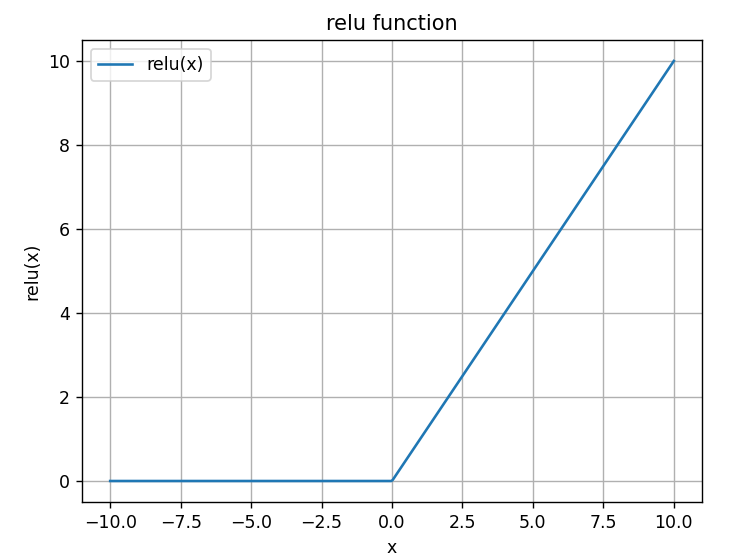
\includegraphics[width = 0.8 \textwidth]{./figures/relu}
  \caption{The ReLU Function}
  \label{fig:red}
\end{figure}


\end{document}